\documentclass[12pt]{article}
\usepackage{sydewkrpt}

%%%%%%%%%%%%%%%%%%%%%%%%%%%%
%%%    Begin Document    %%%
%%%%%%%%%%%%%%%%%%%%%%%%%%%%
\begin{document}
\pagenumbering{roman}

\waterlootitle{Permute-Structures and Methods}{
  SkyGrid Inc.\\
  Engineering Team\\
  Sunnyvale CA.
  }{
  Alexander Huras\\
  \#20340660\\
  2B Systems Design Engineering\\
  May 2012
  }


\begin{waterlooletter}
University of Waterloo\\
Waterloo, ON\\
N2L 3G1

\today

Dr. Paul Fieguth, PhD\\
Department Chair, Systems Design Engineering\\
SkyGrid Inc.\\
University of Waterloo

Dear Dr. Fieguth,

\indent This report, prepared as my 2B work report entitled ``Permute-Structures and Methods'' is an analysis of the efficiency of a particular set of algorithms used for generating sets of permutations,\linebreak[0] and explores a novel algorithm for creating a graph/polytope consisting of permutations as nodes/vertices.
This report will also explore the potential applications of such an abstract data structure, as well as performance limitations and further optimizations of the algorithm, particularly to escape the speed restrictions of its current platform (Ruby with Ruby Graph Library). \\

\indent SkyGrid Inc. makes products that connects people with their interests. Currently SkyGrid develops and maintains a custom news aggregation application of the same name, \linebreak[0] as well as recently, developing an iOS and web platform to deliver socially integrated video through services/social networks such as Facebook and Twitter.
While this report focuses on more abstract concepts and algorithms not explicitly required by the current system, my interest in the topic stemmed (perhaps serendipitously) from my work in the development of the social integration features present in the iOS and web platform, which lead to a greater appreciation for the Graph abstract data structure, particularly in the domain of social networks, and information distribution.
During my time at SkyGrid, I worked closely with Software Engineers Fei Xie, and Jie Hu, as well as CEO Kevin Pomplun.\\

\indent I have prepared the enclosed report ``Permute-Structures and Methods'' as my 2B Work Report for the Engineering team at SkyGrid Inc. \linebreak[0] This report, the third of four work reports that I must submit as part of my degree requirements, and it has not received previous academic credit at this or any other institution.\\

Sincerely,\\
\vspace{1em}

Alexander Huras
20340660

\end{waterlooletter}

\dotableofcontents

\tocsection{Abstract}
Motivated by a desire to visualize self-similar patterns in permutation sequences, a novel algorithm was developed to generate a structured network of permutations.
The approach is evaluated based on performance and computational efficiency, and a soft metric: the quality of the rendered result.
Within the performance analysis, comparisons to outstanding permutation sequence generation algorithms are made, with a focus on ACM 303, a permutation algorithm authored by Ord-Smith in which a lexicographically ordered permutation sequence is generated.
The theoretical performance of the novel algorithm with respect to ACM 303 is found to be lacking (order n!(n-1)!), which leads to an assessment of the visual aspect of the graph.
A series of projections are presented with commentary on visible recursive structure, and it is demonstrated that higher-order permutation networks present a difficult challenge in visualization (using force-directed expansion).
Recommendations to improve the process include a re-implementation of the algorithm in a lower-level language, and utilizing the vast performance of the cloud to handle larger permutation network expansions.
\newpage
\singlespacing

\tocsection{Glossary of Terms}
\textbf{C}---An imperative procedural programming language. Generally used for lower-level programming.\\
\textbf{Cayley Graph}---A graph that encodes the abstract structure of a mathematical ``Group''. A central tool in combinatorial and geometric group theory.\\
\textbf{Compute}---Vernacular, computing power applied for an arbitrary unit of time. Used qualitatively to generally imply a massive amount of computational resources directed at a given problem.\\
\textbf{Edge}---As relating to a Graph, a linkage between a pair of nodes. Edges can be directed, in which case the link has a defined start and end, or undirected, which simply specifies that the link exists.\\
\textbf{Graph}---An abstract data structure representing a set of objects and their interconnections.\\
\textbf{Graph - (adjacency)}---A particular type of Graph, constructed through the use of `Adjacency Lists': a collection of lists (one per Node/Vertex) specifying the existence and direction (if necessary) of the edges associated with the Node/Vertex in question.\\
\textbf{Graph - (directed)}---A particular type of graph consisting entirely of edges that have a defined start and end point. In such a graph the edge \{A,B\} $\neq$ \{B,A\}.\\
\textbf{Hamiltonian}---A descriptor of a Graph, stating the existence of a Hamiltonian Path: A path in an undirected Graph that visits each Node exactly once.\\
\textbf{Haskell}---A purely functional programming language, featuring a \emph{lazy} interpreter, notable in speed relative to C.\\
\textbf{\emph{k}-Order}---Relating to ring-permute structures generated by an input set of size \emph{k}.\\
\textbf{Node}---Also called a \emph{Vertex}: an object forming a Graph, connected to other Nodes by way of Edges.\\
\textbf{Permutation}---A distinct representation of a unique rearrangement of the elements in a set. There exists \emph{k}! such rearrangements of a set of size \emph{k}.\\
\textbf{Permute}---The act of applying a Permutation to a set of elements.\\
\textbf{Permutohedron}---pl. Permutohedra: A geometric body in which all vertices occupy points specified by all the permutations of an initial vector. For example, given the vector (x,y,z)=(1,2,3) the permutohedron would be specified by the set of vertices \{ (1,2,3), (1,3,2), (2,1,3), (2,3,1), (3,1,2), (3,2,1)\}. A notable property of permutohedra is that for an initial \emph{k}-dimensional vector, the body occupies \emph{(k-1)} dimensions.\\
\textbf{Polytope}---A geometric structure consisting entirely of flat sides. A polygon is an example of a Polytope.\\
\textbf{Recursion}---The process of repeating operations in a Self-Similar fashion.\\
\textbf{RGL}---Acronym for Ruby Graph Library, a library of functions and definitions borrowing heavily from the Boost Graph Library, as implemented in C++.\\
\textbf{Ruby}---Ruby is a dynamic object-oriented programming language. It is modern relative to C.\\
\textbf{Self-Similarity}---An object is said to be `Self-Similar' when it is exactly or approximately similar to a part of itself. That is to say, in a general sense, that features of the object taken in isolation, resemble the object in its entirety.\\

\newpage
\doublespacing
\pagenumbering{arabic}
\section{Introduction}
\setlength{\parindent}{1cm}
\subsection{Motivation}
This process began as a desire to efficiently create and visualize permutation networks---structured groupings of the given permutations of a list of elements, while also developing a novel use-case for a more directed transformation of combinatorial geometric constructs.
Similar models exist in the form of permutohedra---(\emph{n}-1)-dimensional geometric bodies (polytopes) whose vertex coordinates are given by the permuted vector (1, 2, 3, ... , \emph{n}).
However, while multi-dimensional polytopes constructed as Cayley Graphs exhibit certain interesting properties (such as being Hamiltonian), \linebreak[0] they do so (especially when the combinatorial polytope exceeds three-dimensions) at the expense of losing their visual interpretability (for humans).
For these purposes a novel method of permuting elements of a set/vector while simultaneously generating a human-readable (displayable in three dimensions) directed graph was developed.\\

The analysis will consist of two elements.
Firstly, establishing the theoretical efficiency of the novel permutation algorithm, with comparison to algorithms referenced in \cite{Ord-Smith:1970}, and \cite{Ord-Smith:1971}, and secondly: technical consideration of the use of the algorithm for permutation-based decision modelling.
While only a specific rule-set was defined for the path the algorithm takes to visit each node in the graph, it is noted that the structures \linebreak[1] created by permutation-centered processes could be altered based on an arbitrary symmetrically consistent rule-set, leading to the generation of other aesthetically pleasing (potentially) or, in a more technical sense---practical (ideally) structures.\\

\pagebreak[2]

\subsection{Metrics}
The \emph{ringPermute} method will be evaluated based on two metrics.
The first: Operational efficiency. The best \emph{ordered} permutation sequence generators are well within the realm of \emph{O(n!)}.
The section of \emph{ringPermute} that generates the permutations should have a similar speed (in terms of computations, not tested speed, after all: Ruby is an interpreted language, and thus is nowhere near as fast as the C, or Assembly processes covered by \cite{Sedgewick:1977}).
It is thus the goal to effectively represent up to \emph{n} = 10, or 3.6 M permutations in network form (graph with size $\approx$ 12 M) within a reasonable time period.
The second: A soft metric---the \emph{ringPermute} structures generated, when rendered, should betray some sense of self-similar symmetry.
This will be discussed further within the analysis section, however because of the inherently self-similar formulation of the factorial function \emph{ $\Pi$ \{ n, n-1, n-2, $\cdots$, 2, 1 \}}, the graph representation of the permutations (at least in structure) should clearly represent incrementally smaller permute-rings.
Due mainly to accessibility, Gephi was used to handle the graph files, and export the rendered versions. \linebreak[0] Gephi is an open-source graph/network visualization program, running on JVM\footnote{For more information on Gephi, and the open-source graph visualization initiative, refer to www.gephi.org}.\\

Constraining these two goals is practical limitation of creating and rendering results.
The generated structures should be \emph{accessible}, that is to say, one should be able to (in isolation, without especially powerful hardware), generate relatively large permute-structures, on a non-purpose built machine (i.e. not a supercomputer).
This applies pressure to the amount of computations required for a given structure, and should be capped in terms of elapsed computation time.
The time required should be less than 30 seconds for a ring-permute structure less than or equal to 8-Order.
This time was chosen as a ballpark figure, from which to base comparisons.
As will become evident, the usefulness of the `30-second' boundary will ultimately play a minor role in evaluating success, as will be demonstrated in figure ~\ref{Performance Table}, no single result is particularly close to being cut-off by the figure.
It is almost fortunate that this is the case however, as the ballpark estimation serves its purpose completely, without requiring a re-evaluation of relevance.\\

\newpage
\subsection{Algorithm}
The algorithm (henceforth ``\emph{ringPermute}'') was developed to generate all the \emph{n}! permutations of a list of \emph{n}-elements, by visiting each unique permutation exactly once.
This forms a permutation sequence, and places it in the category of permutation generation algorithms, such as ACM algorithms: 86, 115, and 323 \cite{Trotter:1962,Peck:1962,Ord-Smith:1968} among others.
It should be noted that \emph{ringPermute} relies heavily on a modified leftRotate function which for convenience was added to Ruby's ``Array'' class\footnote{Due to how interactive Ruby (irb) handles object modification inline, the actual \emph{ringPermute} function employs the use of two versions of leftRotate, namely a soft rotate (where self is not modified) followed by a hard rotate to commit the change to the \emph{self} object.
It is unknown at this time why this particular workaround was necessary.}.
Below are the supplementary functions used in \emph{ringPermute}.\\

\begin{multicols}{2}
\singlespacing
\begin{verbatim}
class Array
  # note function modifies self
  def leftRotate!(i=0, j=self.length-1)
    temp = self[i]
    until i == j do
      self[i] = self[i + 1]
      i += 1
    end
    self[j] = temp
    return self
  end

  def spawnLeftRing(i=0)
    edgeList = []
    j = i
    until j == self.length do
      edgeList.push(self.dup)
      edgeList.push(
              self.leftRotate!(i) )
      j += 1
    end
    return edgeList
  end
end
\end{verbatim}
\end{multicols}

\doublespacing
The \emph{leftRotate!} method cyclically rotates each element in the list, and returns the result.
The \emph{spawnLeftRing} method, in combination with \emph{leftRotate}, creates a clockwise directed loop or ring\footnote{Note, that in the context of this document, \linebreak[0] the ``Ring'' describes a construct within the graph abstract data structure, that when visualized resembles a closed loop or \emph{ring}.
The use of this term in the context of graph visualization does not imply that the set of nodes within the loop are themselves mathematically defined as a ``Ring''.} where within a single execution context, each node is connected to only two-other nodes.\\
\pagebreak[2]

If one were to follow Ring's directed edges, one would visit each node exactly once, before returning to the initial node.
The direction of the cycle is consistent with:\\
\centering
\emph{A $\succ$ B}, where \emph{B = A.leftRotate!}\\
\raggedright
\setlength{\parindent}{1cm}

An example of such a network can be seen below, note the orientation with respect to the direction of rotation, this arbitrary convention will be maintained throughout the examples in this document.
The concept is further demonstrated in figure ~\ref{8-ring}.\\

\begin{figure}[ht]
\centering
\scalebox{0.4}{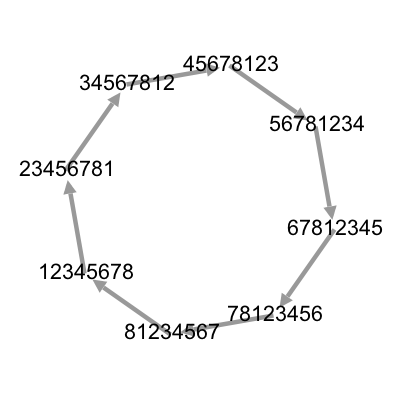
\includegraphics{Graphs/8-ring.png}}
\caption{An oriented ring demonstrating left-rotation.}
\label{8-ring}
\end{figure}
\setlength{\parindent}{1cm}

In the same way that each iteration of calculating a factorial draws upon unit-increasing (or increasing) multiplication, the creation of a ring permutation network involves recursively generating incrementally smaller rings.
However, to ensure that successive ring does not include any duplicate elements (or duplicate elements already in the permutation sequence) the \emph{leftRotate!} method is called with incrementally larger index values.
This is equivalent to only rotating a section of the array.
The \emph{ringPermute} method is shown below.
It is important to recognize that this implementation requires that a directed adjacency graph object be pre-initialized (the \emph{graph} argument).\\

\newpage
\begin{figure}[h]
\centering
\singlespacing
\begin{verbatim}
def ringPermute(set, i=0, edges=[], graph=nil)
  if edges.length >= 2
    until edges.length == 0 do
      x = edges.pop;
      graph.add_edge(edges.pop, x)
    end
  end
  if i == set.length - 2 then
    return set.spawnLeftRing(i)
  else
    (set.length - i).times do
      edges += ringPermute( set.leftRotate(i), i + 1, edges, graph )
      graph.add_edge(set.dup, set.leftRotate!(i)
    end
    return edges
  end
end
\end{verbatim}
\caption{Implementation: \emph{ringPermute}}
\label{ringPermute}
\end{figure}

It should be noted that \emph{ringPermute} utilizes two different calls to \emph{leftRotate}, the more exclamatory ``\emph{leftRotate!}'' as defined earlier performs a hard rotation, by modifying the self object.
When called without the exclamation mark, the function returns a rotated copy of the self object, and leaves the self object unchanged.\\

\newpage
\section{Analysis}
\setlength{\parindent}{1cm}

\subsection{Performance}
While it may be obvious that the algorithm generates edges that imply \emph{n}! unique nodes for the \emph{n}-set input, it is important \linebreak to note that the rotation algorithm that forms the basis for every link is itself \emph{O(k)}, where \emph{k} is the parameter passed to \emph{leftRotate!}.
Furthermore, it may not be useful to describe the performance of a permutation sequence algorithm in terms of `worst-case' scenarios,\linebreak for in every unique execution context of \emph{ringPermute} (i.e\@. not as a result of recursion) the function will perform a constant number of operations, leading to a constant number of nodes and edges.
Thus the number of `operations' performed by the \emph{ringPermute} will be evaluated as a function of the length/size of the argument.\\

As is stated by Sedgewick, the fastest computer permutation algorithms operate by exchanging two elements per permutation \cite{Sedgewick:1977}.
As is immediately apparent by the inclusion of a rotation method (in general, this performs more than a single exchange, and thus anecdotally does not comply with Sedgewick's observation) within \emph{ringPermute}, the algorithm is not optimal.
However as the number of permutations increases, the importance of their \emph{context}, becomes important.
The algorithm's speed will be assessed by the number of combinatorial iterations required to generate the permutation network, as shown in figure ~\ref{ringPermute-Derivation}.
As well as a simple test on one computer to establish whether low-order ring-permute structures can be created in less than 30 seconds.
This is present in figure ~\ref{Performance Table}\\

\hspace{0.5cm}
\begin{figure}[ht]
\onehalfspacing
\centering
\emph{f(n) = $\Pi$ \{ (n)*g(n-1), (n-1)*g(n-2), (n-2)*g(n-3), $\cdots$, 2*g(1) \},}\\
 where g $\equiv$ O( leftRotate!(k) ) = k, k $\epsilon$ $\mathbb{Z}$\\
\emph{f(n) = n * $\Pi$ \{(n-1)(n-1), (n-2)(n-2), ..., 2, 1\}}\\
\emph{f(n) = n!*(n-1)!}
\caption{General performance of \emph{ringPermute}}
\label{ringPermute-Derivation}
\end{figure}
\pagebreak[3]
\doublespacing

As becomes immediately apparent, the use of the rotate method squares the necessary number of loop operations necessary to generate the graph, causing what is already a computationally large problem into one that in all realistic sense is not reasonable for any moderate \emph{n}.
For reference, with \emph{n} = 9, \emph{f(n)} = 14.6-Billion, an unreasonably large number of calculations for such a small \emph{n}.
Compared to leading algorithms such as Ord-Smith's ACM 303 \cite{Ord-Smith:1968}, whose compiler-optimized performance is within the realm of \emph{O(Cn!)}, where \emph{C} is reasonably small, \emph{ringPermute} is (at least theoretically) computational failure.\\
\pagebreak[1]

However, the 30-second benchmark, as seen in figure ~\ref{Performance Table} was met for all structures of 8-Order or less.
 What is alarming however, is the divergence of the elapsed time between 8-, and 9-Order structures.
Ultimately, while the time discrepancy is outstanding in its own right, what is most disturbing is the nonlinear relationship between the size of the created graph, and the amount of time required to produce a marginal node.
Ultimately, this betrays some of the operations necessary to grow graphs with RGL, and could be related to the time required to add a marginal node/edge to the graph data structure.
At this point in time it is unknown  what the relationship between graph size and time elapsed to generate (by implicitly adding nodes) is, and thus could be the subject of additional research.\\

\begin{figure}[ht]
\centering
\hspace{1cm}
\begin{tabular}{| r | r | r | l |}
	\hline
	\emph{n} & Nodes & Edges & Time [s]\\
	\hline \hline
	1 & 1 & 1 & 0.14m \\
	2 & 2 & 2 & 0.15m \\
	3 & 6 & 9 & 0.36m \\
	4 & 24 & 40 & 1.3m \\
	5 & 120 & 205 & 6.9m \\
	6 & 720 & 1,236 & 41.5m \\
	7 & 5,040 & 8,659 & 0.43 \\
	8 & 40,320 & 69,280 & 7.56 \\
	9 & 362,880 & 623,529 & 547 \\
	\hline
\end{tabular}
\caption{Performance Tests on One Computer}
\label{Performance Table}
\end{figure}

\newpage

\subsection{Visualization of ringPermute Structures}
Perhaps in reference to the situation described above, Robert Sedgewick; a prominent computer scientist (heavily referenced within this document) has stated:\\

\begin{quote}
``In short, the fastest possible permutation method is of limited importance in practice. There is nearly always a better way to proceed, and if there is not, the problem becomes really hopeless when \emph{n} is increased only a little''\cite{Sedgewick:1977}\\
\end{quote}

Even within those algorithms compared by Ord-Smith in \cite{Ord-Smith:1970,Ord-Smith:1971}, there is a noted discrepancy between the speed of algorithms designed to generate permutation sequences, and those designed to generate \emph{ordered} permutation sequence.
\pagebreak[1] Intuitively, doing anything other than the bare-minimum number of computations (Sedgewick's `exchanges') should be slower, or rather---require more computations.
This is undoubtably the case with \emph{ringPermute}.
As all rings are directed, and the rule governing their direction is that of rotation (partial or complete), there is a necessary number of extra steps to compute, and that is  reflected by the increased amount of information present in the final result (a directed graph as opposed to a list, or set of permutation vectors).
\pagebreak[2] Thus while \emph{ringPermute} indeed generates an ordered permutation sequence, it also generates a visualizable structure, providing a powerful illustration of a relatively intuitive, recursively generated network.\pagebreak[2]\\

\newpage
\begin{figure}[ht]
\begin{minipage}[b]{0.5\linewidth}
\centering
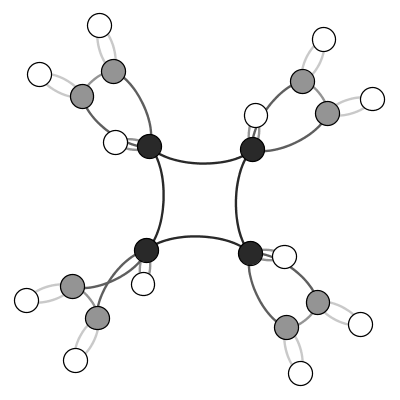
\includegraphics[scale=0.55]{Graphs/4-permute400.png}
\caption{ringPermute: \emph{n} = 4}
\label{ringPermute-4}
\end{minipage}
\hspace{0.5cm}
\begin{minipage}[b]{0.5\linewidth}
\centering
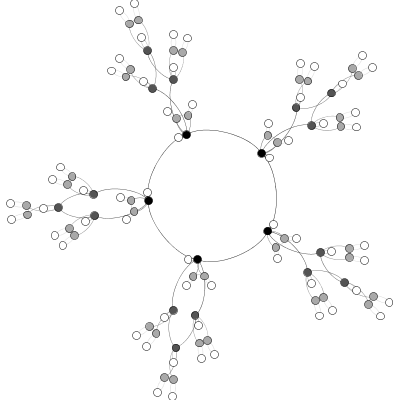
\includegraphics[scale=0.55]{Graphs/5-permute400.png}
\caption{ringPermute: \emph{n} = 5}
\label{ringPermute-5}
\end{minipage}
\end{figure}
\pagebreak[2]

In figures ~\ref{ringPermute-4}, ~\ref{ringPermute-5}, ~\ref{ringPermute-6}, and ~\ref{ringPermute-7} we see ideal use-cases of the ring-permute structure.
Within these figures, the darker nodes represent a larger inDegree.
A fact that may not be immediately apparent from the algorithmic creation of the ring-permute structure, is for a structure of order \emph{n}, (that is to say, generated from a set of size \emph{n}), the inDegree of the root nodes (all complete rotations of the source node) is \emph{(n-1)}.
This property arises from the fact that for any ring of \emph{k} nodes, the vertices will themselves be members of a ring with \emph{(k-1)} nodes (down to zero).
This relationship is shared by the factorial function itself.
\pagebreak[0]
By way of this being visually apparent within maps of smaller (\emph{n} $\leq$ 8) structures, this is a positive outcome of the visualization experiment.
At the (noticeable) expense of computation time, the result is clear, and in certain cases, aesthetically pleasing.\\

For larger structures, such as in figure ~\ref{ringPermute-7}, or most exemplar: figure ~\ref{ringPermute-8}, the elegance of the visual aspect becomes more difficult to render under the current framework.
This is an almost unavoidable circumstance as the number of nodes to be displayed begins to overwhelm the big-picture \footnote{For example, the difference in size (nodes + edges) between figure ~\ref{ringPermute-8} and a 9-order ring-permute structure is roughly 1-million elements ($\approx$ 100x times larger).} and with it, the symmetries most obvious in a 6-order structure.
This represents a significant challenge in generating larger structures, but there exists an equally demanding challenge (if not more so) in presenting or rendering them visually\footnote{For all cases demonstrated within the context of this document, the use of graph-visualization tools powered by (in part) the results of an implementation of Yifan Hu's graph coarsening algorithm\cite{Hu:2006}}.

\begin{figure}[ht]
\hspace{0.5cm}
\begin{minipage}[b]{0.5\linewidth}
\centering
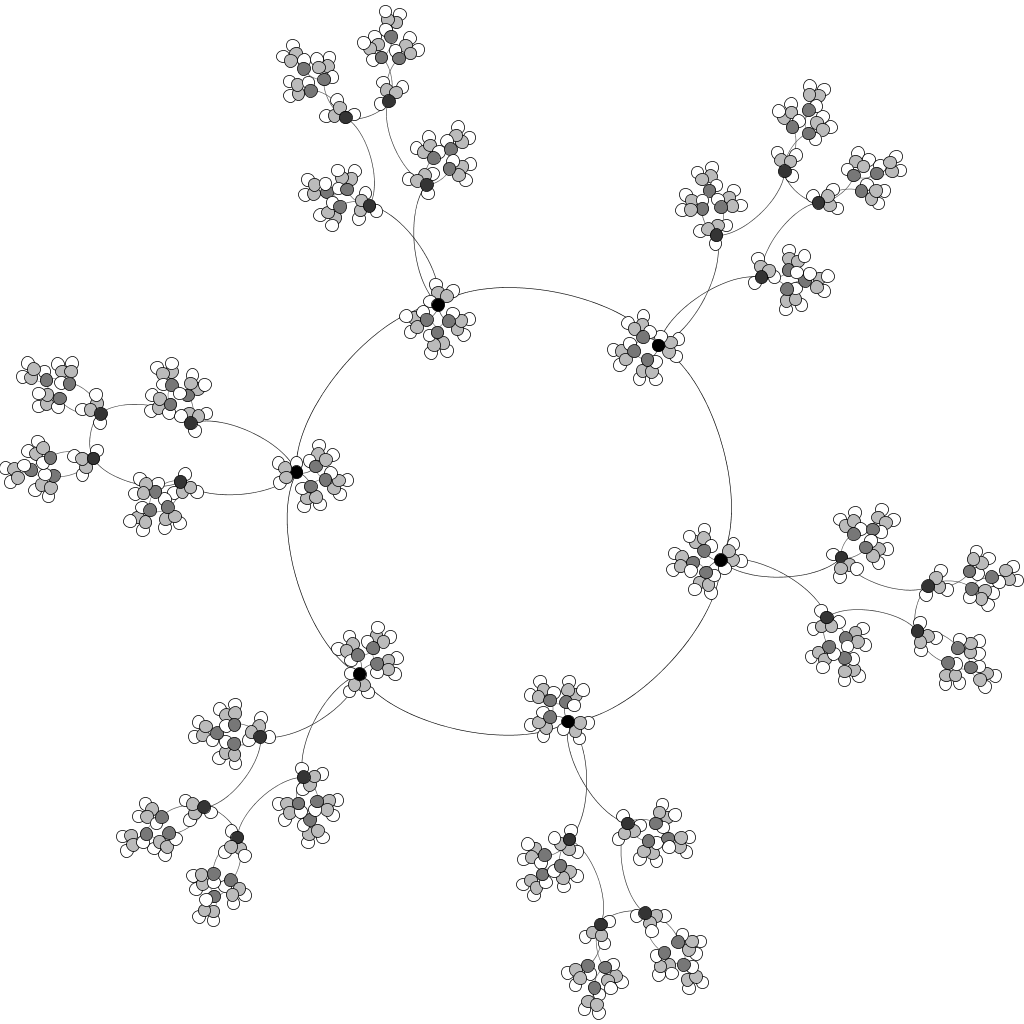
\includegraphics[scale=0.15]{Graphs/6-permute.png}
\caption{ringPermute: \emph{n} = 6}
\label{ringPermute-6}
\end{minipage}
\hspace{0.5cm}
\begin{minipage}[b]{0.5\linewidth}
\centering
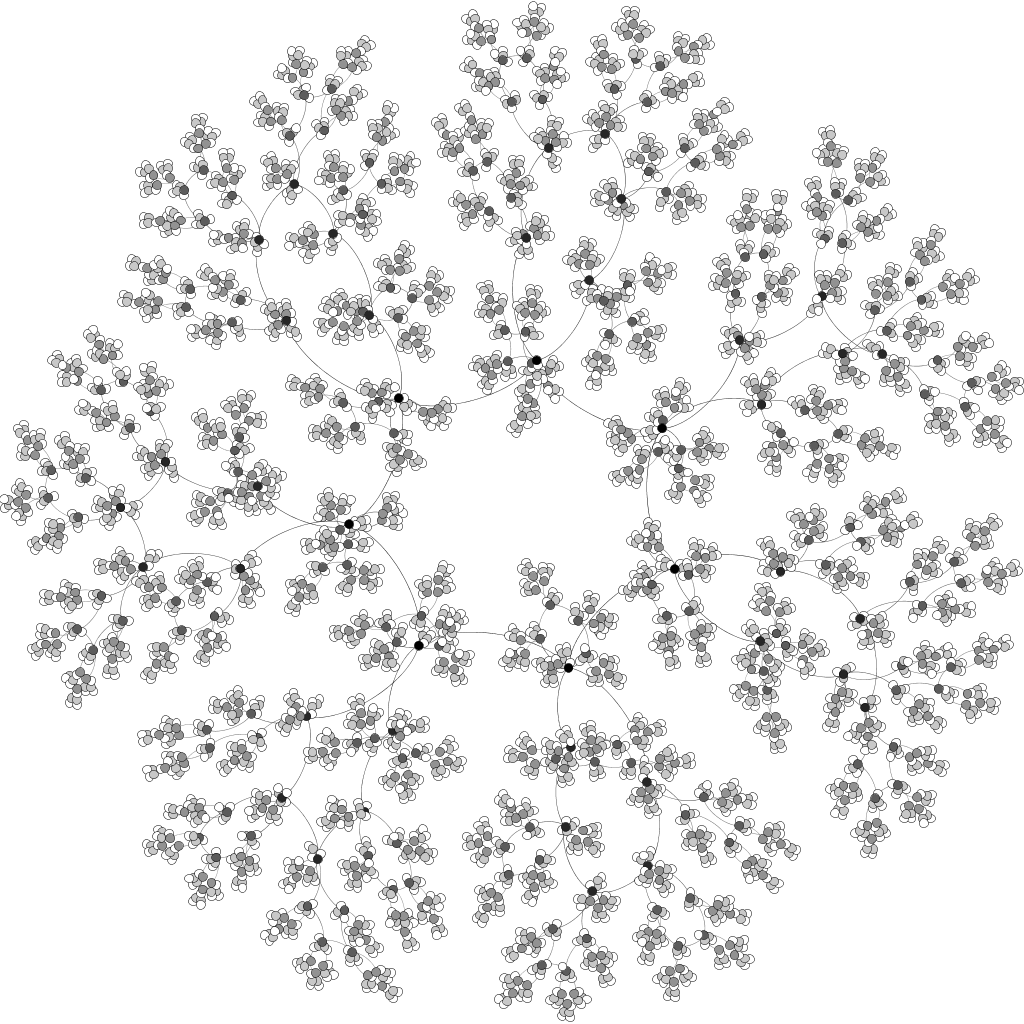
\includegraphics[scale=0.15]{Graphs/7-permute1024.png}
\caption{ringPermute: \emph{n} = 7}
\label{ringPermute-7}
\end{minipage}
\end{figure}

\begin{figure}[ht]
\hspace{0.5cm}
\centering
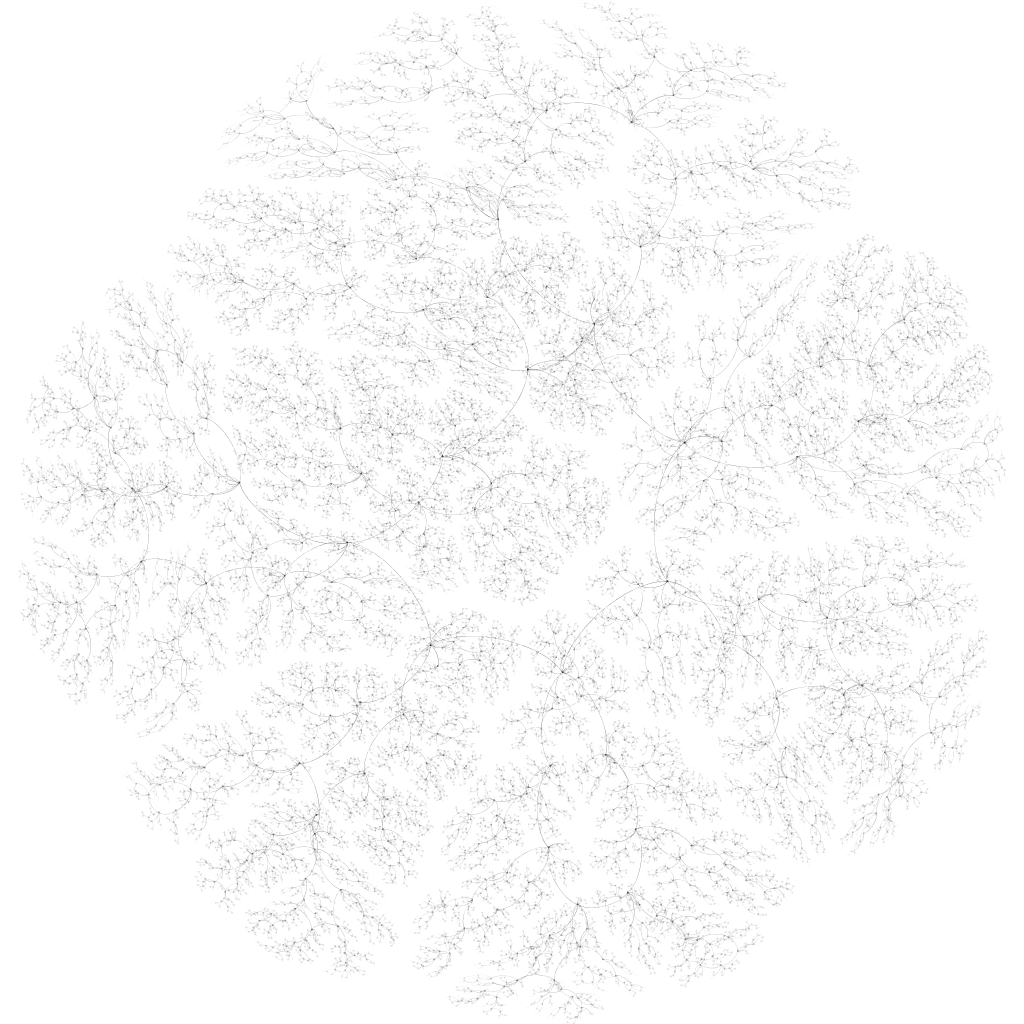
\includegraphics[scale=0.25]{Graphs/8-permute.png}
\caption{ringPermute: \emph{n} = 8}
\label{ringPermute-8}
\end{figure}
\pagebreak[4]

\subsection{Applications of ringPermute Structures}
The use of permutation sequences has become increasingly relevant as an alternative to traditional statistical tests of trend.
Particularly \emph{exact}-tests which have seen an uptick in prevalence as an alternative test that guarantees preservation of type-I error \cite{Corcoran_Mehta_2001}.
Typically more computationally expensive to run, with the advent of more efficient permutation generators, these tests have gained increased relevance. While ringPermute has been shown to be nowhere near the most efficient algorithm for purposefully generating complete permutation sequences, the algorithm does generate a particularly novel data structure which could be used to approximate decision scenarios typically handled in decision trees, or probabilistic matrices. \\

The usefulness of a permutation structure within the context of pseudo-random permutation selection is possible if the algorithm is extended (or limited) in such a way that the orientation of a given permute-ring can be established through arbitrarily specific rules (such as a particular arrangement of rotation cycles).
For example, in the case of decision tree modelling (statistical or otherwise), it is useful to suggest a probabilistic edge weight consistent with the likelihood that the next step in the process/tree-traversal (i.e\@. following a Hamiltonian cycle) will match an arbitrary rule (such as rotation).
If one were to simulate a decision process based on the statistically most likely series of data transformations (each corresponding to a node in the permute-structure),  the generation of a purpose built data structure could be useful. In the aforementioned case, within a simulation routine one-need only evaluate the nearest (to an arbitrarily deep level, with a maximum of \emph{n}) \emph{k}-permute-rings, and probabilistically traverse the graph---generating further permute-rings when necessary based on each successive edge-traversal.
In this way, while the existing nodes in the ring-permutation structure do not themselves form a complete permutation cycle, the performance loss associated with creating a marginal ring-permutation (avoiding the factorial problem) can be avoided.\\

In general the graph abstract data structure has many significant performance limitations when evaluating arbitrarily deep paths.
This can be avoided by only evaluating what is needed within a permute-network.\\
\pagebreak[3]
Within recent years the need/desire to aesthetically visualize complex networks has increased\cite{Lima:2011}.
While rendering times are characteristically high, the ring-permute structure---particularly at higher orders exhibits pseudo-fractal/self-repeating patterns, that might prove interesting to explore.
Thus, to satiate curiosity, this structure may expose some relationships not immediately obvious. Knowledge for knowledge's sake.\\

\newpage
\section{Conclusions}
\setlength{\parindent}{1cm}
\subsection{Performance}
The algorithm exhibits \emph{O(n!*(n-1)!)} runtime performance, which is roughly a factor of \emph{n}! slower than the fastest permutation sequence generators.
This combined with the large space overhead required to store the graph generated make it a poor choice for a pure permutation generator.
However, while under the current schema of generating the structure, it is possible to implement the algorithm in a lower-level language such as C, or Haskell; which by virtue of more direct hardware interfacing, can be used to speed up the process by as much as three-orders of magnitude.
However, within practical considerations (particularly under the pretense of elegantly displaying the permute-structures) the Ruby environment is sufficient for \emph{ringPermute} calls where \emph{n} $\leq$ 8.\\

\subsection{Visual Interpretability}
A soft metric, the ability to interpret the graph was defined as an easily identifiable recursive symmetry---the ability to resolve all the individual ring-permute structures.
This is most obvious in figures ~\ref{ringPermute-4},  ~\ref{ringPermute-5}, and ~\ref{ringPermute-6}, but the granularity is lost for \emph{n} $\textgreater$ 7. A more chaotic example can be found in Appendix A, where the result is not as clearly resolved (partially due to having over three-hundred thousand nodes, and partially because the calculations required to arrange said nodes in anything other than a swirling tangle of edges is beyond the grasp of my current hardware under Gephi).
An understandable consequence of the factorial growth pattern, the goal was to effectively visualize structures of order 10 or higher.
In this the algorithm running under its current environment has failed.
However, this is in part due to the technical problems faced in the rendering of the networks.
Currently even using highly-efficient Yifan Hu force-directed graph drawing algorithms \cite{Hu:2006} in Gephi\footnote{As well as others for presentation, such as Force ATLAS.}, the hardware limitations of the rendering system are too great to elegantly display over 9\@! nodes.\\

\newpage
\section{Recommendations}
\setlength{\parindent}{1cm}
\subsection{Performance}
As discussed earlier, due to the large overhead required to run Ruby with RGL (Ruby Graph Library\footnote{rgl.rubyforge.com}), it is recommended that the algorithm be ported to C++, or Haskell.
The boost graph library in C++ is mature, lightweight, and very efficient, leading to arguably the best tool for graph creation.
Furthermore, if we wish to set our sights higher, nVidia's CUDA platform is enticing, and the existing C++ code could be augmented with a GPU coprocessing module.
However, if the results from the visualization experiment are to be taken into account, it is unlikely that (at least under the current setup) the mere act of generating the structure is the bottleneck.
At some point, graph coarsening, or some other as yet unknown tool for effectively arranging the elements of the network must be used.
At a primitive level, the act of generating the graph is trivial compared to the at of rendering images.
This in and of itself is of concern if the end goal is to visualize the networks.
Ultimately, if partial decision tree modelling is a priority, then visualization does not factor into the equation, and the processes behind generating the ring-permute structures has only to be committed.\\
\pagebreak[1]

\subsection{Visualization}
As the size of the permutation network increases (and in congress, the marginal rate of increase), the problem of effective visualization becomes non-trivial.
Ultimately, there must come a point when the human viewer does not \emph{need} to see every single node, but rather the overarching patterns, or symmetries.
While figure ~\ref{ringPermute-8} fails as an elegant visualization compared to figure ~\ref{ringPermute-5}, the juxtaposition of the two may not result in a relevant comparison.
The comparison doesn't carry as much weight, primarily because the method of visualization doesn't scale at the same rate that the factorial growth function. \pagebreak[2]
Throughout this document many examples of ring-permute structures have been displayed, and it should be obvious that the growth of the permutation network is \emph{fast}.
The argument can be made that the reason the comparison between figures ~\ref{ringPermute-4} and ~\ref{ringPermute-8} is invalid is because the scale discrepancy between the two is outrageous.
A 4-order \emph{ringPermute} has just 24 nodes; compared to the relatively massive 40,320 nodes of an 8-order structure.
In this particular case, a doubling of the input length, results in an almost 2,000x increase in size of the result.
This again brings us back to the factorial nature of the problem.
The factorial increases faster than all polynomial and exponential functions (excluding double exponential), so this represents a major challenge in displaying these networks.\\
For \emph{small n}, the problem can be faced by simply applying more compute. With the rather economical availability of resources like Amazon EC2, one can with relative ease overcome local issues such as a slow processor, or not enough RAM.
However, for \emph{large n} the growth becomes overwhelming, and brings us back to Sedgewick's initial statement (paraphrased), if we \emph{really} need to generate permutations for \emph{n} $\approx$ 3,000, we are doing something wrong.\\

\newpage
\onehalfspacing
\addcontentsline{toc}{section}{References}

\bibliographystyle{IEEEtran}

\bibliography{bib}

\newpage

\tocsection{Appendix A --- 9-order ringPermute}
\label{Appendix A}
A rather large permute structure, with 362,880 nodes and 623,529 edges, this is close to the limit of what is possible to display in Gephi.
A telling sign being the rather organic-looking structure generated by a graph-coarsening algorithm.
Gone is the very clear symmetry present in figure ~\ref{ringPermute-7}, and the clear macroscopic structure in figure ~\ref{ringPermute-8}.\\
\hspace{0.5cm}
\centering
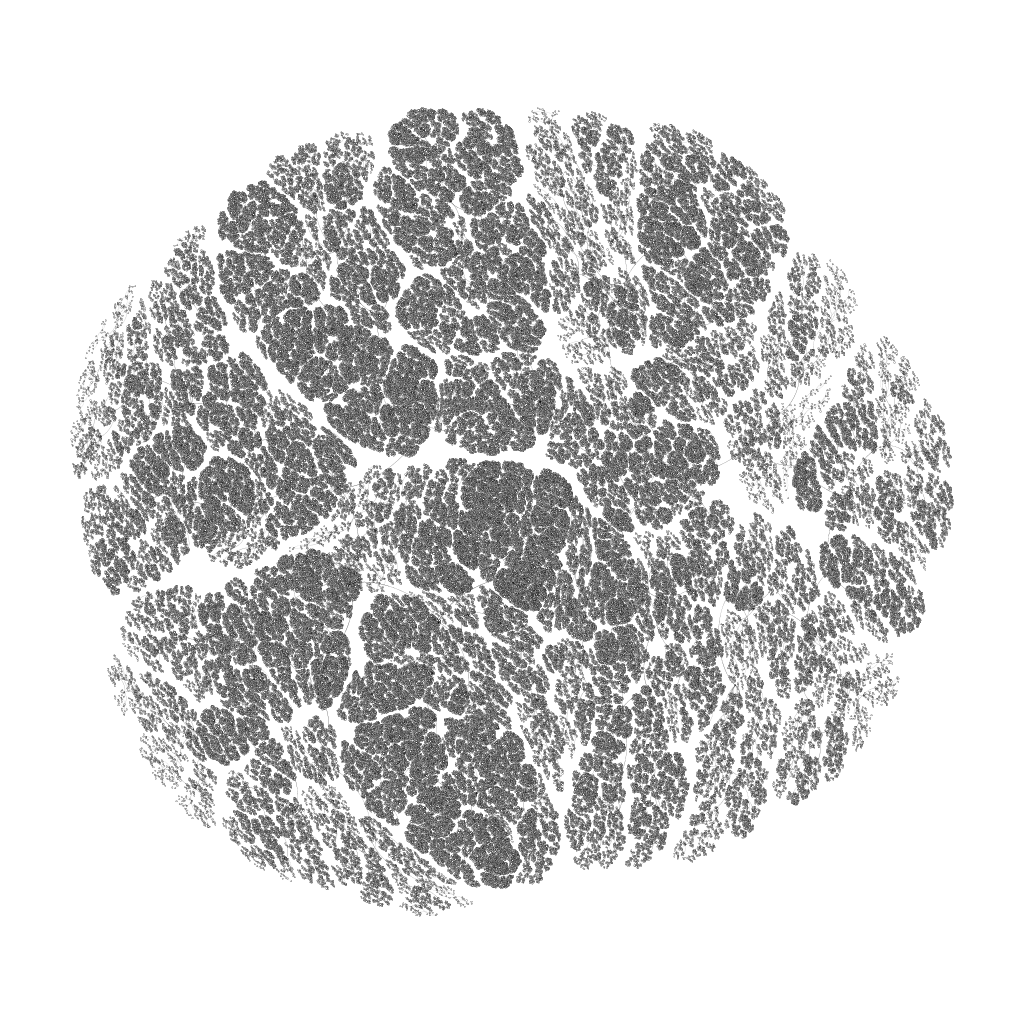
\includegraphics[scale=0.45]{Graphs/9-permute1024.png}

\end{document}
